\section{Air traffic and emissions distribution}
The previous section discussed the forces of flight and the generation and dispersion of aircraft emissions, from the perspective of a single aircraft. However, the state of the atmosphere is inhomogeneous with respect to space and time, meaning that the climate sensitivity to aircraft emissions differs considerably, depending on the time and location of their release. Furthermore, in airspace regions where traffic density is high, aircraft fly in close proximity and their exhaust plumes may intersect, giving rise to nonlinear local climate effects that must also be considered in aviation climate analysis. Therefore it is useful to explore the influence of air traffic management and spatial and temporal demand on the distribution of air traffic, and hence its associated emissions. 

\subsection{Air traffic management}
Air traffic management (ATM) is the system of services responsible for overseeing the network-wide implementation of safe, orderly and efficient air traffic flows, providing assistance to aircraft in transit from departure to destination aerodrome. It is the role of the air traffic control (ATC) team to manage and monitor air traffic in their respective airspace in real time, ensuring that optimum safety, order and efficiency of aircraft operations are maintained at all times \cite{SecretariatGeneral2016}. 

%This means that air traffic controllers must constantly monitor the state of the airspace, swiftly identifying and resolving any unfavourable circumstances by issuing the appropriate clearances or instructions to rectify the situation. 

\subsubsection{Air traffic safety} 
The inherent risk involved in the transportation of vast numbers of passengers at near transonic speeds through the upper atmosphere means that aviation safety is of paramount importance. A safe aircraft operation takes the path of least danger, primarily influenced by the need to avoid unfavourable atmospheric conditions and to prevent conflicts with other aircraft \cite{Zhang2012, Baumgartner2007}. In-flight atmospheric conditions susceptible to icing, turbulence or the presence of hazardous convective weather can all be classified as unfavourable for aircraft, with the latter presenting the greatest constraint on aircraft routing \cite{Mitchell2006, Krozel2007}. The increased risk resulting from flight through weather-affected regions means that aircraft must re-route, leading to restrictions on available airspace and deviations from the optimal flight profile, thus increasing flight-times, fuel burn and delays \cite{weather_delay_2021}.

The safety risks associated with aircraft-to-aircraft collisions necessitate air traffic controllers to impose safe separation standards between aircraft in the lateral, longitudinal and vertical direction, as specified in \cite{ICAOPANSDoc44442016}. The stated minimum separation distances between aircraft are 5 nautical miles (NM) laterally, 20 NM longitudinally and 1,000 ft in the vertical direction under the most lenient scenarios. A breach of separation laws in more than one direction is known as a conflict and must be resolved as quickly as possible. The enforcement of separation minima therefore introduces a theoretical upper limit on airspace density, i.e. the number of aircraft that occupy a fixed volume of airspace at any one time. 

\subsubsection{Air traffic order} 
To keep air traffic flows organised within controlled airspace, aircraft are ordered to follow the traditional fixed-route air traffic network, constructed from four key airspace elements that facilitate the air traffic management process \cite{SecretariatGeneral2016}:

\begin{itemize}
\item \textbf{airports/aerodromes} - an area of land or water intended to be used for the arrival, departure and surface movement of aircraft;
\item \textbf{waypoints} - a specified geographical location used to define the flight path of an aircraft, representing either a navigational aid (navaid) or a reference coordinate that the aircraft must fly by or fly over;
\item \textbf{airways} - a controlled portion of airspace established in the form of a corridor (usually 8-10NM wide) between two waypoints;
\item \textbf{sectors} - a region of airspace managed by a single ATC team, stratified into various levels to accommodate a wide variety of traffic.
\end{itemize}

In \cite{Odoni1987}, the notion of optimising air traffic flows for a given demand and capacity is explored, in which air traffic flows are represented using these four key elements. \textbf{Airports} represent the sources and sinks of the flow, \textbf{airways} are the arcs along which the flow travels, \textbf{waypoints} are the network nodes at which airways intersect, merge or diverge, and \textbf{sectors} are a collection of waypoints and contiguous segments of airways. The fixed-route network restricts airspace availability even further, due to the discretisation of flight levels and the requirement to pass specified waypoints \cite{Bilimoria1996, FAA2017}. This can lead to particularly high frequencies of aircraft passing through high-density airspace, potentially leading to congestion along busy airways and waypoints where airways intersect resulting in inhomogeneities in the distribution of air traffic and potential congestion along high-density airways.

%The fixed-route network further restricts airspace availability due to the discretisation of flight levels and the requirement to pass specified waypoints \cite{}. Although it is thought that available airspace does not constrain the flow of air traffic directly \cite{}, it is likely to have an effect on potential air traffic flow congestion in high demand airspace regions, due to the limitations imposed on potential trajectories to be flown by aircraft in controlled airspace. Increases in local congestion can lead to further inhomogeneities in the distribution of air traffic and associated emissions.

%Examples of high-density airspace due to fixed route airspace?

\subsubsection{Air traffic efficiency}
The third and final component of effective air traffic management is the optimisation of flight trajectories, subject to the prioritisation of safety and the compliance with the fixed-route airspace structure. Flight trajectory optimisation is an essential step in ensuring maximum airspace utilisation and efficiency, so that revenue is maximised and demand levels are sufficiently met. Trajectory optimisation is a multi-faceted problem, requiring consideration of nonlinear aircraft performance, wind and weather forecasts, payload, departure fuel load, reserve fuel load and ATM constraints that restrict aircraft operations and routing \cite{Soler2015}. This requires an exhaustive assessment to be carried out at the flight planning stage, to test all possible combinations of route, payload, fuel load and operating approach, involving tens to hundreds of thousands of calculations per flight. The most optimal scenarios are then ranked in order of optimality, with the final route selected based on operator preference and/or the occurrence of unexpected circumstances, such as sudden adverse weather conditions or aircraft conflicts \cite{Altus}.

In an ideal airspace situation where the atmosphere is calm and constant; aircraft are not constrained to a fixed route; and there is no risk of conflict with other aircraft, the least-time and least-energy aircraft operation would be to fly the great-circle arc between departure and destination. The vertical profile of the aircraft would consist of a continuous climb out to the most efficient cruise altitude, then to cruise at constant speed, with the ability to cruise-climb continuously as the aircraft burns fuel and loses mass. In reality, the true optimal route can deviate considerably from the great-circle arc, instead taking the path which minimises the risk of bad weather encounters and collisions, abides by the fixed-route airspace structure, whilst also flying a route which is optimised with respect to wind and temperature. The magnitude and direction of wind and the localised variation in temperature experienced by the aircraft throughout flight, can have a drastic impact on route optimality, with tailwinds and colder temperature regions being favourable \cite{Murrieta-Mendoza2014}. Ng et al.\ (2012) \cite{Ng2012} found for a wide range of wind-optimal flight scenarios that domestic flights saved up to 3\%, and international flights saving up to 10\% on both fuel burn and travel time, despite flying longer routes. Furthermore, the vertical flight profile of the aircraft must adhere to flight level allocations, meaning that step climbs must be performed as fuel is burnt, further condensing air traffic and its corresponding emissions into narrow bands of altitude. 

\subsubsection{Airspace capacity}
The effective management of air traffic relies on the human cognition of air traffic controllers to make difficult decisions and carry out complex tasks in a time-critical dynamic environment. This includes ensuring safety through avoidance of poor atmospheric conditions and conflicts with other aircraft, maintaining order by flying along the fixed-route airspace network, and optimising air traffic flows with respect to wind and weather. As density and complexity levels of air traffic increase, so does the mental workload of the air traffic controller, up until a threshold level is reached where the controller can no longer safely handle the situation. The maximum number of aircraft permitted by the ATC team in charge of a particular airspace volume is known as the airspace capacity, and is driven by the airspace situation, state of equipment being used, and the controller's own mental state \cite{Majumdar2004}. Airspace capacity is limited more by controller workload than is it separation laws, meaning human cognition is the true limiting factor on the number of aircraft that can occupy a particular airspace volume at a particular time \cite{Welch2007, Bilimoria1996}. Therefore, models of controller workload are often used to estimate airspace capacity, in which ATC tasks are modelled to determine a safe upper limit on workload. In Welch et al.\ (2007) \cite{Welch2007}, a macroscopic workload model is proposed which generalises ATC tasks into four distinct categories: background, transition, recurring and conflict tasks. This provides an objective basis for estimating capacity and enables the formulation of an analytical relationship between airspace capacity and sector volume, as seen in figure \ref{cap_vs_vol}.

%The effective management of air traffic relies on the human cognition of air traffic controllers to make difficult decisions and carry out complex tasks in a time-critical dynamic environment. As density and complexity levels of air traffic increase, so does the mental workload of the air traffic controller, up until a threshold level is reached where the controller can no longer safely handle the situation and design capacity is reached. Therefore, threshold mental workload is a key determinant of airspace capacity and is driven by the airspace situation, state of equipment being used, and the controller's own mental state \cite{Majumdar2004}. To estimate capacity, controller workload models are used, which model ATC tasks to determine a safe upper limit on workload. In \cite{Welch2007}, a macroscopic workload model is proposed which generalises ATC tasks into four distinct categories: background, transition, recurring and conflict tasks. This provides an objective basis for estimating capacity and enables the formulation of an analytical relationship between airspace capacity and sector volume, as seen in figure \ref{cap_vs_vol}.

\begin{figure}[H]
  \centering
  \includegraphics[width=0.65\linewidth]{cap_vs_vol.pdf}
  \caption{Aircraft capacity estimation against sector volume for a range of airspace scenarios \cite{Welch2007}. E refers to the length to width ratio of the sector, \ce{G_b}, \ce{\tau_C}, \ce{\tau_r} and \ce{\tau_r} are all empirical parameters related to controller workload, P is the mean task recurrence period per aircraft, T is the sector transit time, \ce{M_h} and \ce{M_v} are the designated horizontal and vertical separation minima between aircraft within the sector and E[\ce{V_{21}}] is the typical aircraft closing speed \cite{Andrews1997}.}
  \label{cap_vs_vol}
\end{figure}

The capacity estimation model from figure \ref{cap_vs_vol} predicts that, for a 10,000~NM$^3$ rectangular sector of dimensions 156~NM (length, ratio 4:1) $\times$ 39~NM (width) $\times$ 10,000~ft (height), a maximum of 16 aircraft may be present at any one time. In a purely hypothetical situation where separation laws dictate capacity and all aircraft are travelling in one direction lengthways, the sector could support a maximum of 490 aircraft, assuming a separation of 5~NM laterally, 20~NM longitudinally and 1,000~ft vertically. This emphasizes the sheer extent to which human factors limit the ability to maximise capacity, and highlights the need for airspace modernisation to increase automation, integration and collaboration in the ATM system, enabling the further increase in capacity levels towards minimum separation capacity \cite{Gardi2016}. 

%This is based on the assumption of two opposing traffic streams travelling lengthwise through the sector, with 72\% (\textasciitilde12) travelling in one direction and 28\% (\textasciitilde4) travelling the other, all at a speed of 550 knots (kt). 

%Assuming that each aircraft is travelling in a similar direction and is spaced equally apart, one possible scenario would be two rows of eight aircraft, as seen in figure \ref{cap_example}. Each aircraft would be separated up to 50 NM laterally and 25 NM longitudinally. In a hypothetical situation where separation laws dictate capacity, this airspace volume would support up to 100 aircraft spread 5 NM apart laterally and 20 NM longitudinally, further emphasizing the extent to which human factors limit the ability to maximise capacity. To highlight the plume overlap potential of maximum capacity airspace, plume dimension estimates from Kraabol et al. (2000) \cite{Kraabol2000} are overlaid onto figure \ref{cap_example}. Using plume dimension estimates from figure \ref{} and the capacity model from figure \ref{cap_vs_vol}, maximum plume overlap scenarios can be inferred.



% Write more about cap vs vol diagram, saying about what it means for distance between aircraft. How this lines up with Schlager ideally.

%In the observation of plume-scale climate effects in high-density airspace regions, airspace capacity is an important concept;  The overlapping of plumes can lead to the superposition of emissions entrained within them. This gives rise to the saturation of climate forcing species in the surrounding atmosphere, further accentuating nonlinear plume-scale climate processes that occur, as elaborated on in section \ref{Plume-scale climate effects}. % Using plume dimension estimates from figure \ref{} and the capacity model from figure \ref{cap_vs_vol}, maximum plume overlap scenarios can be inferred.


%Flight routes are constrained by the need to avoid hazardous situations, abide by ATC standards and optimise aircraft operations, however another factor which significantly affects air traffic distribution is aviation demand. There are inconsistencies in the levels of demand for aviation both geographically and temporally, depending on the demographic of the area and the preferences of those who fly \cite{}.

\subsection{Global air traffic and emissions distribution}
The nature of air traffic and emissions distribution was investigated in Olsen et al.\ (2013) \cite{Olsen2013} where a range of global aircraft emissions datasets are compared (NASA-Boeing 1992, NASA-Boeing 1999, QUANTIFY 2000, Aero2k 2002, AEDT 2006 and aviation fuel usage estimates from the International Energy Agency) to show distribution patterns in the latitudinal, longitudinal and vertical sense. Further to this, temporal variations with respect to both the diurnal (time of day) and seasonal (time of year) cycles are explored.

\begin{figure}[H]
  \centering
  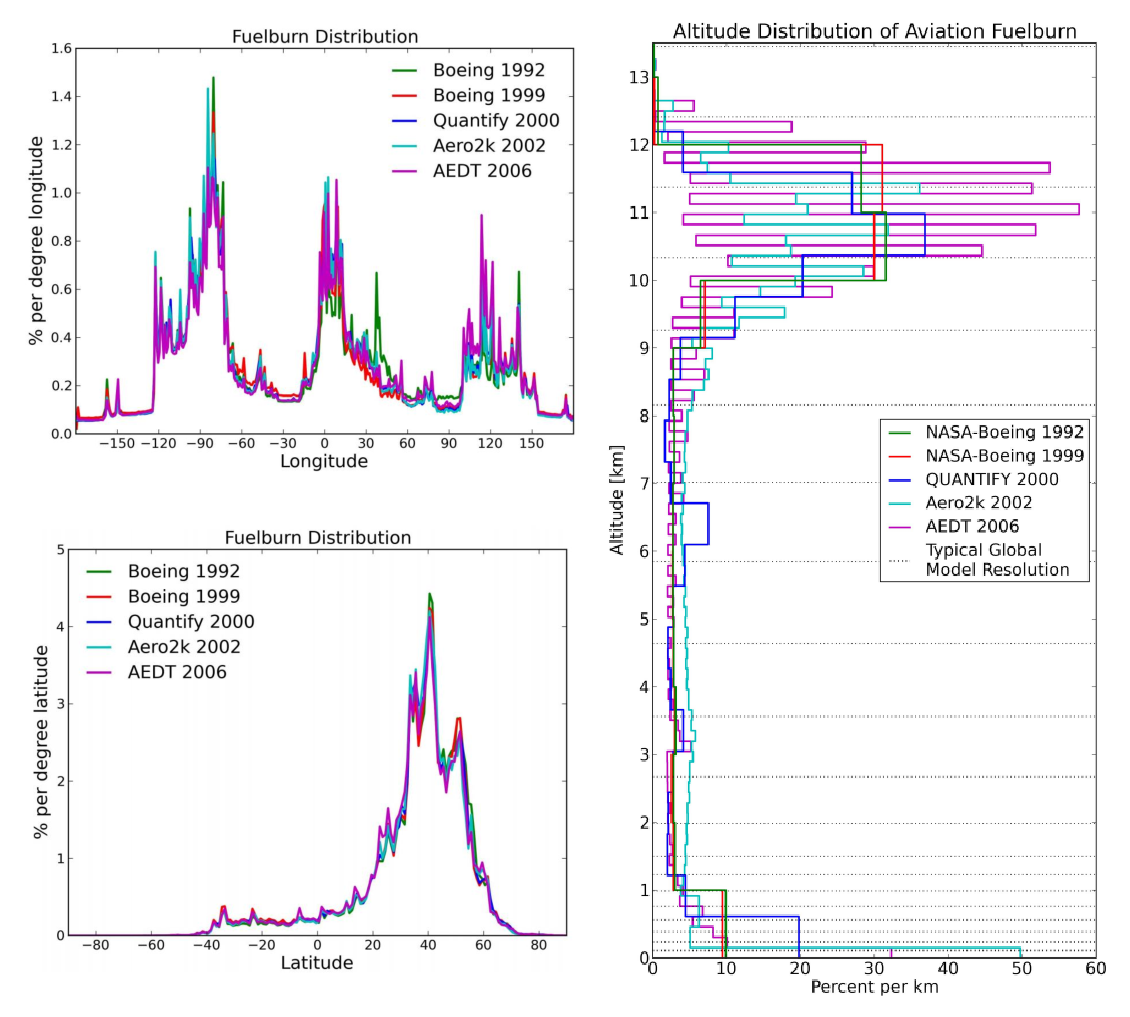
\includegraphics[width=0.8\linewidth]{FB_dist_spatial.pdf}
  \caption{Spatial (latitude, longitude and altitude) distribution of global aviation fuel burn from a range of aircraft emissions datasets \cite{Olsen2013}.}
  \label{FB_dist_spatial}
\end{figure}

The climate sensitivity of the atmosphere is highly variable depending on the exact latitude, longitude and altitude combination, because of the spatially varying chemical and meteorological state of the atmosphere (e.g. \cite{Houghton2001, Inness2013, Emmons2000}). Accurate accounting of spatial distribution patterns of air traffic is therefore very important in the estimation of aviation climate impact. Figure \ref{FB_dist_spatial} shows the spatial distribution of fuel burn across the range of datasets in the longitudinal, latitudinal and vertical directions. The longitudinal distribution shows three emissions peaks around the densely-populated regions of the US, Europe and East Asia, with the largest situated above the North American land mass. It is evident in the latitudinal distribution, that the Northern Hemisphere dominates, with a strong peak in the northern mid-latitudes that appears due to high volumes of air traffic above the US and Europe, as well as along the connecting region of airspace, the North Atlantic flight corridor (NAFC). Contrarily, there are almost no emissions present in southern latitudes below 40\textdegree~S, with the region between 40\textdegree~S and the equator constituting only a small percentage. The altitudinal distribution on the other hand, experiences emissions peaks around both the low altitude LTO area and the high-altitude cruising regions between 9 and 13~km, with relatively low emission intensities at mid-altitudes. Furthermore, the peak around cruising altitude is discretised into peaks every other flight level, due to the vertical separation constraints and the allocation of aircraft to specific flight levels, thus owing to further increases in emissions intensities at these altitudes.

%Similarly, Wasiuk et al.\ (2016) \cite{Wasiuk2016} derived global \ce{NO_x} emissions totals for 2005 to 2011 by coupling an aircraft emissions modelling framework with an air traffic dataset for this period. Aircraft performance was modelled for each flight in the dataset using the BADA3 method \cite{Nuic2010} and the emissions were calculated using the BFFM2 \cite{DuBois2006}. Figure \ref{Wasiuk_fig} portrays the spatial distribution of \ce{NO_x} emissions on a latitude-longitude map averaged over the six year period. For both altitude bands, main areas of aviation activity such as flights over mainland and popular flight corridors are highlighted. The outcome of this analysis suggests similar findings to that of Olsen et al. for both the latitude and longitude plots in figure \ref{FB_dist_spatial}. In the longitude plots in figure \ref{Wasiuk_fig}, the three main areas of activity remain prominent; mainland US, Europe and East Asia, along with the much more distinguishable flight corridors that connect these regions. In the latitude plots, the Northern Hemispheric skew is also present, with most air traffic remaining within 20 to 60\textdegree N and a peak occurring around 40\textdegree N.

%\begin{figure}[H]
%  \centering
%  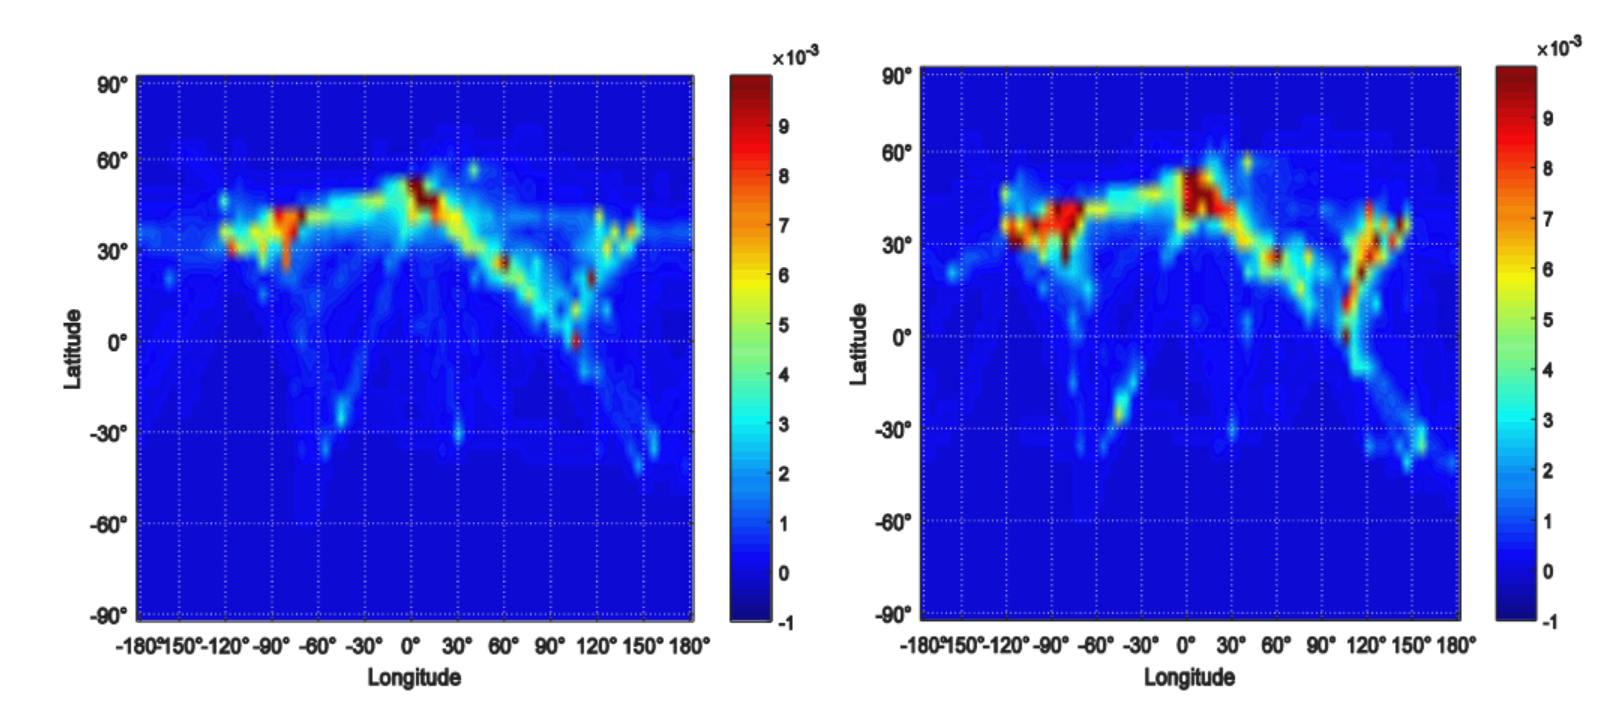
\includegraphics[width=\linewidth]{Wasiuk_fig.png}
%  \caption{}
%  \label{Wasiuk_fig}
%\end{figure}

The presence of diurnal and seasonal variations in key chemical and meteorogical parameters throughout the atmosphere has been widely investigated in the literature (e.g. \cite{Schanz2021}). The diurnal and seasonal variation in aviation fuel burn from Olsen et al.\ (2013) \cite{Olsen2013} is displayed in figure \ref{FB_dist_temporal}. The temporal fluctuations in both the state of the atmosphere and the distribution of fuel burn and emissions allude to the fact that the climate sensitivity to aircraft emissions is always changing, and therefore these parameters must be under constant observation to ensure accurate determination of global climate effects from aviation. The diurnal cycle of global aviation fuel burn, as seen on the left hand side of figure \ref{FB_dist_temporal} displays a peak at around 15:00~UTC, which decreases through the night until around 09:00~UTC where total fuel burn begins to increase again. With regards to seasonal variation, there is significant variance between emissions datasets, however in general, all display a wintertime minimum between December and January, and a summertime maximum between June and September.

\begin{figure}[H]
  \centering
  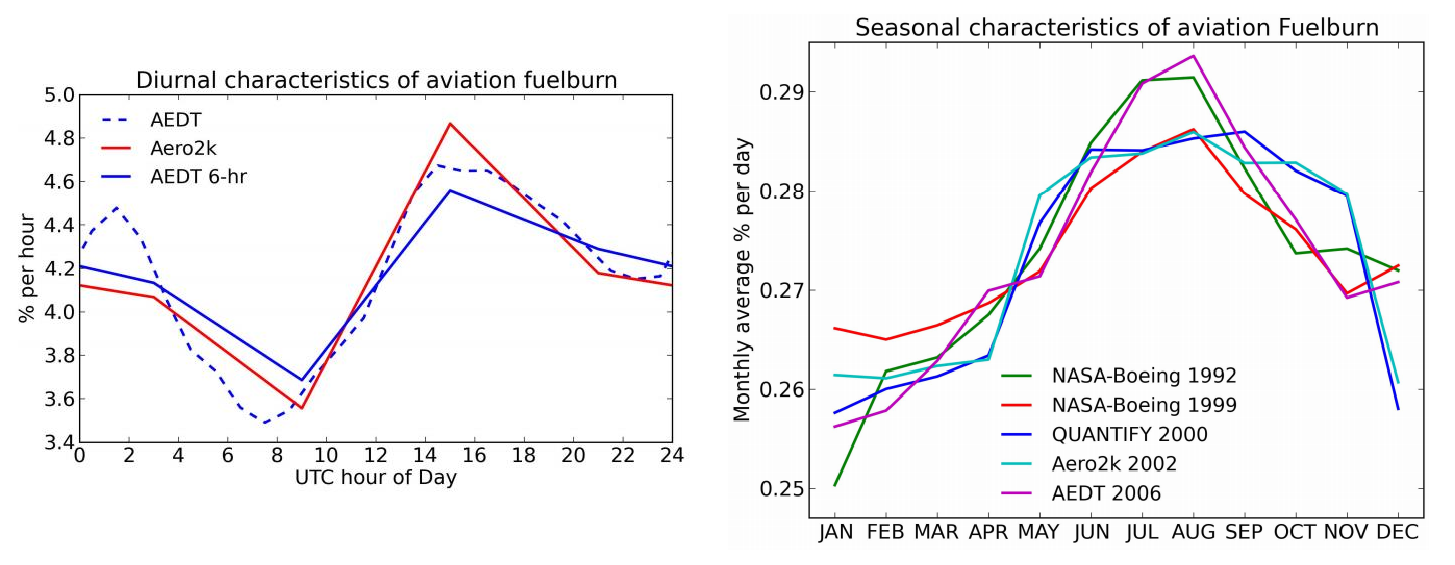
\includegraphics[width=0.8\linewidth]{FB_dist_temporal.pdf}
  \caption{Temporal (diurnal and seasonal) distribution of global aviation fuel burn expressed as percentage from a range of aircraft emissions datasets \cite{Olsen2013}.}
  \label{FB_dist_temporal}
\end{figure}

\subsection{Local air traffic and emissions distribution}
Due to the fixed-route nature of airspace, aircraft tend to fly along common airways or flight corridors, and pass common waypoints along their journey, leading to exceptionally high flux densities of aircraft through these regions at peak times. This has implications on the nonlinear chemical and physical effects occurring at the plume scale, due to the intersection of aircraft plumes and the elevated exhaust gas concentrations entrained within them. A prime example of a high-density airspace region is the NAFC, made up of a series of tracks that aircraft traversing the North Atlantic must follow, updated daily to allow for convective weather avoidance, tracking of the North Atlantic Jet Stream and favourable tailwinds to maximise efficiency \cite{NOTAMS}. The annually-averaged number of aircraft traversing the NAFC per day has increased from 800 in 1997 \cite{Karcher1998} to around 2,500 in recent years \cite{NATS_NAFC}, owing to the tripling of passenger demand since then \cite{World_databank}. With North Atlantic air traffic being confined to a limited number of tracks (usually three or four), it can be assumed that aircraft separation distances and airspace capacities are pushed to their limit on a regular basis along this and other popular flight corridors around the world.

%Schlager figure here

Previous experimental work on air traffic emissions in the NAFC was carried out in the late 1990's, through campaigns such as the Pollution from Aircraft Emissions in the North Atlantic Flight Corridor (POLINAT) and Subsonic Assessment Ozone and Nitrogen Oxide Experiment (SONEX) \cite{Schumann2000}. At least 20 follow up papers were published following these campaigns, in which POLINAT/SONEX data are utilised to provide insight on a number of major scientific issues \cite{Thompson2000}. A noteworthy publication with regards to localised emissions impacts is Schlager et al.\ (1997) \cite{Schlager1997}, which carries out an in-situ investigation of air traffic emissions signatures (nitrogen oxides (\ce{NO_x}), sulphur dioxide (\ce{SO_2}) and cloud condensation nuclei (CCN)) in the NAFC using experimental data from a POLINAT research flight. The research aircraft flew perpendicular to the major eastbound corridor tracks and took measurements of various chemical concentration fields and meteorological parameters throughout. The results show that the superposition of aircraft exhaust plumes led to peak concentrations of \ce{NO_x}, \ce{SO_2} and CCN above background levels by factors of 30, 5 and 3, respectively. This is because plume dispersion timescales greatly exceed the daily frequency with which aircraft emissions are input into the flight corridor, resulting in an inhomogeneous concentration field with narrow and sharp peaks over a relatively low and smooth background level \cite{Schumann2000}.

\begin{figure}[H]
  \centering
  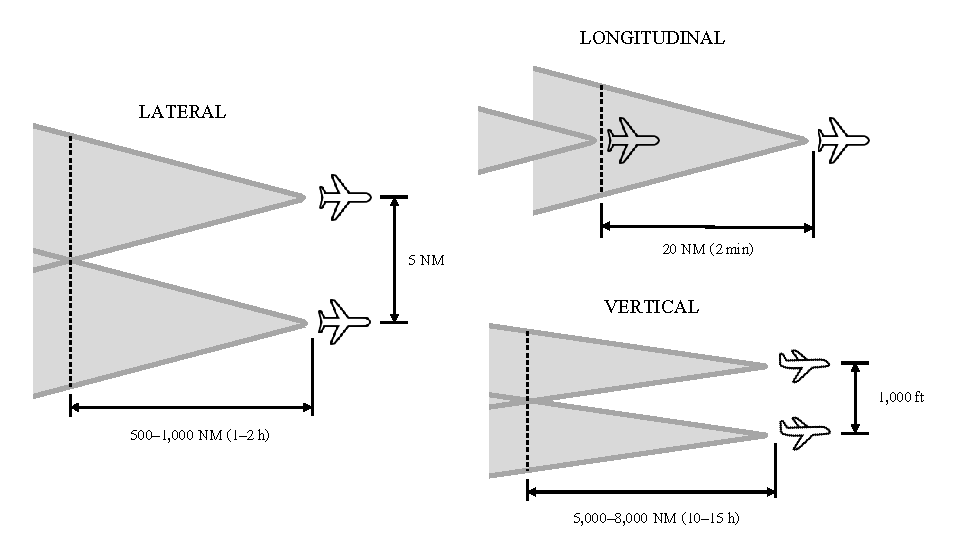
\includegraphics[width=0.9\linewidth]{cap_example.pdf}
  \caption{Lateral, longitudinal and vertical maximum plume overlap scenarios, based on nominal separation minima \cite{ICAOPANSDoc44442016}}
  \label{cap_example} 
\end{figure}

In the observation of plume-scale climate effects in high-density airspace regions, aircraft separation minima determine the minimum possible distance between aircraft and hence the maximum possible overlap between aircraft exhaust plumes. The degree of plume overlap influences the magnitude of emissions saturation, further accentuating nonlinear plume-scale climate processes that occur, as elaborated on in section \ref{Saturation}. Using plume dimension estimates from Kraabol et al.\ (2000a) \cite{Kraabol2000a}, maximum plume overlap scenarios can be inferred. Figure \ref{cap_example} displays the lateral, longitudinal and vertical maximum overlap scenarios for aircraft cruising at 550~kt. The longitudinal separation scenario proves to be the most effective formation for superimposing aircraft plumes, with the intersection time simply equalling the time taken to travel the separation distance between the two aircraft. For lateral and vertical superposition, the intersection time is much longer, as it is determined by the plume expansion rate in that particular direction, up until the midpoint between the two aircraft is reached. For lateral plume overlap to occur, the plumes must expand horizontally to a radius of 2.5~NM (15,190~ft), whereas for vertical, the distance is a mere 500~ft. Despite the drastic reduction in distance, the vertical plume overlap takes about an order of magnitude longer than lateral, because vertical plume expansion is substantially suppressed in comparison due to stable atmospheric stratification counteracting vertical motion \cite{Schumann1995}. In reality, air traffic flows are much more complex and the controlled and orderly formations shown in figure \ref{cap_example} are unlikely to occur naturally. However, the premise still holds that plume overlap occurs most frequently in congested flight corridors such as the NAFC, when aircraft travel along similar tracks and the vertical displacement between aircraft is minimal. 

The importance of safety, order and efficiency in the air traffic management process and the characteristics of global and local air traffic flows have been discussed. As the following section will explore, the atmospheric response to aviation emissions is highly sensitive to time and location, because the instantaneous state of the atmosphere (i.e. the chemical composition and meteorological situation at that particular time and position) determines the production, loss and radiative response of key chemical species that induce climatic effects \cite{Jacobson2005}. With insight into how air traffic and emissions are dispersed locally and distributed globally, the contribution of aircraft emissions to climate change can be more rigorously evaluated.

 %on a global and local scale, through evaluation of the climate forcing mechanisms that result from emissions and analysis of their relative global warming contributions. 

%Further to this, the nonlinear chemistry and microphysics within the exhaust plume is covered in great detail. % < Probably needs some work.

%Based on 1997 market analysis, it was found that the annually-averaged number of aircraft traversing the NAFC per day is 800 \cite{Karcher_1998}, around FL350 with a cross sectional area of 2000km$^2$. This corresponds to one aircraft passing a fixed point along the corridor every 100s or so. Accounting for the fact that air traffic is confined to a small number of tracks (usually 3 or 4) within the corridor, and that air traffic passenger demand has tripled since then, it can be safely assumed that aircraft separation distances are close to minimum and airspace capacities are pushed to their limit on a regular basis. \cite{Schlager_1997} carries out an in-situ investigation of air traffic emissions signatures in the NAFC, and 

%Using a standard plume distribution and assuming aircraft are separated at a minimum distance in all three directions, worst-case plume overlap scenarios can be deduced. which serve as a theoretical foundation for studies observing the effects associated with multiple overlapping plumes.





